\documentclass[oribibl]{llncs}
 
\usepackage{amssymb} % AMS Fonts
\usepackage{amsmath} % AMSLaTeX
\usepackage{url}
\usepackage[pdftex]{graphicx}

% Compile only with pdfLaTeX
\usepackage[pdftex]{graphicx}

%\reversemarginpar
\makeatletter
\@twosidefalse
\makeatother

\textwidth180mm
\hoffset-30mm

\bibliographystyle{alpha}

\begin{document}

\title{ Skip Lists, Treaps, and Other Randomized Data Structures for Maintaining Ordered Sets}

\author{Bairong Lei, Michael Wexler}

\institute{University of Waterloo, David R. Cheriton School of Computer Science}

\maketitle

\begin{abstract}
  In this project, we will discuss several randomized data structures for maintaining ordered sets. These
  data structures use probabalistic methods to remain approximately balanced, which helps to avoid skewed distributions that can lead to excessive running times. 
\end{abstract}

%%%%%%%%%%%%%%%%%%%%%%%%%%%%%%%%%%%%%%%%%%%%%%%%%%

\section{Introduction}

The need for ordered sets is very common in computer science. By ordered set, we mean a typical set data structure (which provides membership information) which has the additional property of maintaining the order of its elements. At a minimum, an ordered set should contain the functions {\it insert}, {\it contains}, {\it delete}, and {\it successor}. Programmers often need such a structure in order to determine if a given element is in the set, and also to find the nearest successor of a given element. Given the functionality of an ordered set, it can be extended so that every key maps to a certain value. This would essentially be a dictionary data structure. One would hope that the most common dictionary operations would take $O(\log{n})$, or better yet, $O(1)$ time.

There has been much work in developing dictionary data structures that provide fast runtime. Examples of these are hash-tables and binary-search-trees. Hash-tables actually provide $O(1)$ lookup time, compared to binary-search-trees which have $O(\log{n})$ lookup time in the average-case. However, hash-tables are not ordered, so they do not provide the {\it successor} operation. On the other hand, binary-search-trees are ordered, so they are able to provide $O(\log{n})$ time for the successor operation.
 
For binary-search-trees, there is often the occurence where a certain sequence of operations cause the data structure to be skewed. For instance, for a given $n$, if we were to insert the sequence $1, 2, \dots, n$ into a normal binary search tree, we would end up having a very skewed structure, which would could take $O(n)$ time to find an element. For this reason self-adjusting binary-search-trees, such as AVL trees \cite{avl_tree} and red-black trees \cite{red_black_trees}, have been developed. They use deterministic methods to perform self-balancing, so the skewed distribution cannot occur.

The afforementioned data structures, in their classical implementations, all use deterministic methods for organizing their data.  Oftentimes, one can use randomization in order to avoid situations where their data structure becomes skewed. In this paper we will discuss various data structures that use randomization in order to maintain approximate balance.

This paper is organized as follows: section \ref{sctn:randomized_data_structures} will give an overview on several probabalistic set data structures. Section \ref{sctn:implementation} will discuss several of the implementations that we have written. Section \ref{sctn:experiment} will give an overview on some experiments we performed in order to compare these data structures. The last section draws a conclusion of our work.

All test files and program code we describe in this report can be found in our \textsc{GitHub} repository \url{https://github.com/wexlermi/cs840project}.

%%%%%%%%%%%%%%%%%%%%%%%%%%%%%%%%%%%%%%%%%%%%%%%%%%

\section{Randomized data structures}
\label{sctn:randomized_data_structures}

\subsection{Treaps}
The first randomized data structure we will discuss is the treap \cite{Aragon1989}. Treaps are at their foundation binary-search-trees, with a certain amount of randomness that allows them to remain balanced in the average case. Every element in a treap has the binary-search-tree property, such that all the nodes in its right subtree are greater than the root, and all the nodes in its left subtree are less than the root. However, every node in a treap contains a priority value, in which the priority of a treap node is always higher than that of its children. When we insert a new element into the treap, we randomly assign it a priority, which is a random integer from a sufficiently large range to ensure there are no collisions. Then we put the element in the treap, in the place it would go if it were considered only as a binary search tree. Once it is put in its proper place in the treap, a sequence of rotations are performed to restore the priority requirement, while still maintaining proper place to make sure its key is in the proper order.

To search for an element in a treap, we can simply use the binary-search-tree search algorithm.

\begin{figure}[here]
\center
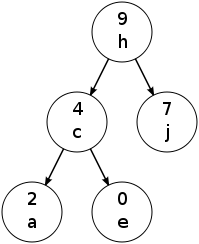
\includegraphics[width=7cm]{images/treap}
\caption{Example of a treap from http://en.wikipedia.org/wiki/File:TreapAlphaKey.svg}
\label{fig:treap}
\end{figure}

Figure \ref{fig:treap} is an example of a very small treap. The letters represent keys, and have the in-order property one would expect in a binary search tree. The numbers represent the priorities. In this case we have a max-heap, since each node has a priority which is a number greater than its children.

\subsection{Skip lists}
A skip-list \cite{skip_list} is a randomized data structure that is inherently built upon linked-lists. Imagine we had a linked list of $n$ elements, in sorted order. If we had to search for an element $x$ in this linked-list, it would be quite inefficient to linearly search for it. To resolve this issue, we can create a linked-list above it which consists of every other element, or every 3rd element, etc. This way, when searching for an element, we can first search through the top level, and once we find an element greater than it, we can drop down and search our original linked list.

We can repeat the process for the top linked list: make a linked-list which consists of every other element in the linked-list below. We keep repeating this process, where each higher level has half the elements of the level below it, until we get a level which has 1 or 2 elements. Then when we search for an element x, we start at the top list, skipping over elements that are less, then dropping down to lower and lower levels, repeating the process, until we either find the element we are looking for, or reach the bottom level and overshoot it, in which case we determine that the element does not exist in the skip list.

Skip-lists use probabalistic methods in order to determine how many levels of a skip-list a given element can be found on. We specify a varible $p$ which represents the probability that an element $x$ on level $i$ will appear on level $i+1$. Every element appears on level 0, as we go to higher levels, we will find less and less elements. The typical value of $p$ is $\frac{1}{2}$. Every time we would like to insert a key $x$ into the skip-list, we first put it at level 0. Then, we "flip a coin" repeatedly, and while we are getting heads, we keep adding $x$ to higher and higher levels, until we get a tails, in which case we stop. This will mathematically ensure that our skip-list has approximately half the number of nodes at higher and higher levels, for $p=\frac{1}{2}$.

Figure \ref{fig:skip_list} is an example skip list. Notice how each level has fewer nodes as we go higher and higher in the skip list. If we were to search for the element 13, we would start at the top level, and go to the right to 17, in which case we have overshot it. Then we drop down to the second level, on node 7, and go to the right to 14. Drop down to the bottom level, and head to 12 to 13. Notice how skip lists allow us to skip over many nodes, giving us an enormous performance increase as compared to an ordinary sorted linked-list, especially when the amount of elements gets large.

\begin{figure}[here]
\center
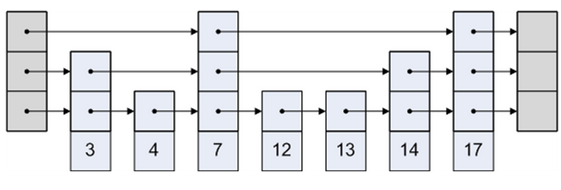
\includegraphics[width=7cm]{images/skip_list1}
\caption{Example of a skip-list from \cite{skip_list}}
\label{fig:skip_list}
\end{figure}

\subsection{Skip lifts}

In \cite{skip_lift} Bose, Douïeb, Morin write about an improvement to the skip list called the skip lift. A skip lift is a skip list in which every element only has the top two nodes. The rest are deleted. Copies of elements which are at the same level are connected by their left and right pointers. Also, the two copies of an elemented have up and down pointers which connect to each other. In Figure \ref{fig:skiplist_vs_skiplift}, we see a visual representation of the skip list (a) vs. the skip lift (b). Notice how the skip lift uses much less nodes than the skip list. The skip lift also has the property that if no nodes appear in a certain level, it will be empty except for the sentinel element which acts as the header.


\begin{figure}[here]
\center
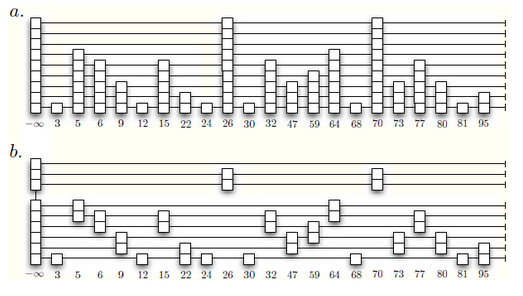
\includegraphics[width=12cm]{images/skiplist_vs_skiplift}
\caption{Skip-list (a)  vs. skip-lift (b)}
\label{fig:skiplist_vs_skiplift}
\end{figure}


\subsection{Jump lists}

Jump-lists \cite{jump_list} are sorted linked-lists, in which case search is expedited by putting "jump" pointers on several nodes, which serve as an "express-lane" for searching. During the course of this project, we came across three variations of the jumplist data structure. These three types of jumplists differ by their methods of establishing the jump links for each node in the list. In the original paper \cite{jump_list}, a jumplist is a sorted single or double linked list. This linked list is a circular linked list with an empty value header. Each node has a key value and a next pointer to connect its immediate successor. Meanwhile, each node has a jump pointer that enables it to jump over several of its successors to reach one of its successors. The link between a node and the target node its jump pointer points to is known as an arch. The arch of the header node of the jumplist is called the {\it fundamental arch}. The jump pointers are created as follows: The node pointed by the jump pointer of the header of the list is selected randomly amongst the rest of the nodes of the list. This assignment splits the list into two independent sublists which are built recursively using the same random procedure. During this construction, the jump pointers do not cross each other. Each node of this jumplist can have more than one incoming jump pointers, but have only one jump pointer pointing to its successor.

The second variation of the jumplist data structure is found in \cite{skip_lift}. It has most of the same features as the jumplist featured in \cite{jump_list}. It maintains the core feature that the jump pointers do not cross over each other. Meanwhile, it ensures that each node has at most one jump pointer being pointed to it and only one jump pointer pointing to its successor. Figure \ref{fig:jumplist} depicts a sample randomized jumplist with 21 nodes.


\begin{figure}[here]
\center
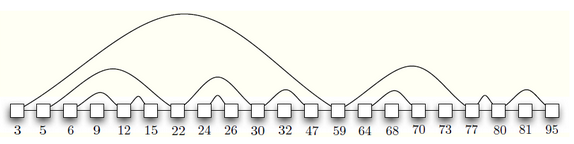
\includegraphics[width=15cm]{images/jumplist}
\caption{A randomized jumplist with 21 nodes}
\label{fig:jumplist}
\end{figure}


The third variation of the jumplist data structure comes from \cite{ElmasryMarch2005}. Like the jumplist introduced by the original randomized jumplist paper, its jumplist maintains the set of common features such as the fact that jump pointers can not cross over each other. However, when the jump pointers are created for the jumplist, the procedure first selects the median node as the node pointed by the jump pointer of the jump list. This fundamental arch divides the whole list into two sublists evenly. These two sublists are then further split evenly and independently using the same process until it reaches the smallest sublists that have only one node and make its jump pointers point to itself. This process builds what they refer to as a {\it perfect jumplist}. Figure \ref{fig:jumplist1} depicts an example of a perfect jumplist with 23 elements.


\begin{figure}[here]
\center
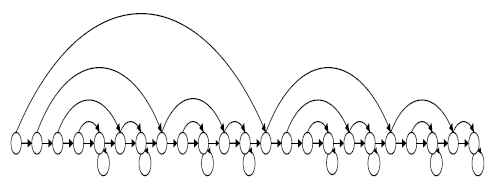
\includegraphics[width=12cm]{images/perfect_jumplist}
\caption{A perfect jumplist with 23 elements}
\label{fig:jumplist1}
\end{figure}

\subsection{Skynet}

Skynet is a scalable overlay network data-structure designed to eliminate the disadvantages of peer-to-peer systems that have no control of data storage location and do not satisfy the need to restrain the routing path within a certain range. Due to the limited time for this project, and the complexity of this data-structure, we were unable to implement SkyNet, but instead we will give a brief overview of the design of SkyNet.

\begin{figure}[here]
\center\underline{}
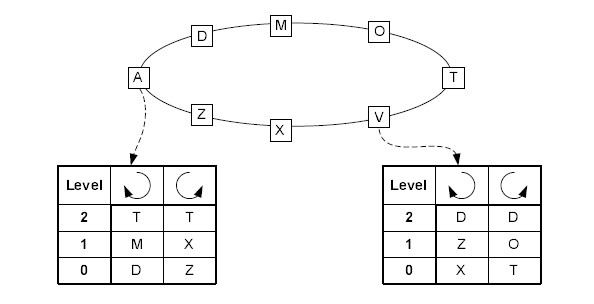
\includegraphics[width=12cm]{images/skynet}
\caption{A Skynet with 8 elements}
\label{fig:skynet}
\end{figure}

Essentially, the structure of the Skynet is a circular double linked list. Each of node of this ring structure has a name ID field which is known as the data record key. From Figure \ref{fig:skynet}, we can see a Skynet structure \cite{skip_net} with eight nodes, each of which has an alphabetic character. Each Skynet node store $2\log{N}$ pointers, where $N$ is the number of nodes in this structure. The pointers facilitate a set of rings as paths for routing through nodes in the rings to search an item. Figure \ref{fig:skynet1} demonstrates the same Skynet of Figure \ref{fig:skynet}, which shows a diverse set of rings by selecting nodes of every level to establish interconnections. For example, from the root ring, we may choose nodes of A, M, T and X to form a subring for the level 1 overlay. We may also further select nodes of A, T and M, X to form two subrings for level 2 overlay from its upper level ring. We continue to use this process to form smaller and smaller subrings until each node only has itself as the new ring. Meanwhile, each node is assigned a numeric ID representing the routing path to reach it.

\subsubsection{Routing in the SkyNet:}

Routing can follow a clockwise direction or a counter-clockwise direction. There are two routing approaches to support lexicographic searching. One approach is called {\it Routing by name ID}. For example, if we need to search node V from node A, this methodology begins routing from Ring 00. Since there are only nodes A and T in Ring 00, it goes down one level to level 1 to route around the subring formed with nodes A, M, T and X. At this moment, we can find node V, so it goes down one level to the level 0 to route around the root ring and eventually find the node V. Another routing approach is called {\it Routing by numeric ID}. There is a hash function that transfers the key of the target item into its corresponding numeric ID. Using the same example to search for node V, the hash function transfers the key V into 111. Therefore, to search node V from node A, the first digit of the numeric ID 111 is 1 and guides the routing from the root ring to the right subring Ring 1 in level 1. Then the second digit 1 directs the routing to the right subring Ring 11 in level 2. Eventually the last digit 1 guides the search routing to the right subring Ring 111 in level 3 and find the target node V. The run time for both Routing by name ID and numeric ID is $O(\log{n})$, where $n$ is the number of the nodes.  Potential future work for this structure can be implementing the insertion and deletion methods.

\begin{figure}[here]
\center
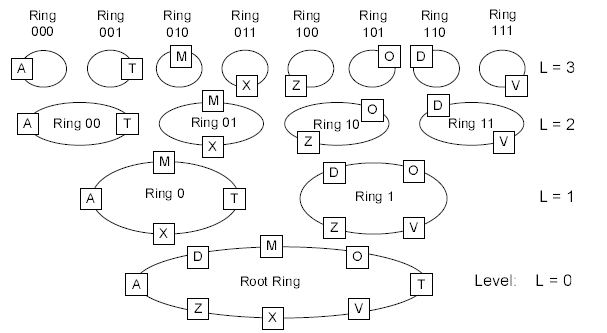
\includegraphics[width=12cm]{images/skynet1}
\caption{A ring hierarchy for an 8-node Skynet}
\label{fig:skynet1}
\end{figure}


\section{Implementation}
\label{sctn:implementation}

For this project, we decided to implement the skip lift \cite{skip_lift}. We built our implementation off an implementation of the skip list \cite{skip_list_imp}. We also implemented the jump list\cite{jump_list}.  Our implementations can be found on our GitHub here: \url{http://github.com/wexlermi/cs840project}.

Due to the limited time for this project, we were unable to implement the operations of {\it delete} and {\it successor}. We were unfortunately only able to implement {\it insert} and {\it contains}, which are the minimum operations a set data structure must contain.

For the experiment we utilized previous implementations of the Treap \cite{treap_imp} and the AVL Tree \cite{avl_tree_imp}.

 \section{Experiment and Analysis}
\label{sctn:experiment}

We thought it would be interesting to collect metrics on runtime and datasize of these probabilistic data structures, to see which ones perform most competitively from a time and space performance perspective. Since the AVL tree is deterministic, we decided to also measure the performance of it, and to use that as a baseline.

For our experiment, we generated a test data set of one million randomly chosen integers. This data-set exists in our GitHub with the name "testdata.txt". For each of our data structures, we measured the timing it would take to insert all the test data into the data structure, as well as the space occupied in memory of the data structure. Also, we made a random permutation of the elements in our data set, which represents a sequence of requests. For this sequence of requests, we measured the time it took to query all the elements for each data structure. Our timing results are in Table \ref{table:timings}.

\begin{table}[htbp]
\caption{Timings for each data structure in seconds}
\begin{center}
\begin{tabular}{|r|r|r|r|r|r|}
\hline
Data Structure & Time to insert (s) & Time to query (s) \\ \hline
AVLTree & 1.462 & 1.227 \\ \hline
Treap &  2.745 & 2.101 \\ \hline
SkipList & 2.610 & 2.789 \\ \hline
SkipLift & 4.106 & 5.835  \\ \hline
JumpList & 4.056 & 4.919 \\ \hline
\end{tabular}
\end{center}
\label{table:timings}
\end{table}

\begin{table}[htbp]
\caption{Space occupied by the data structures in megabytes}
\begin{center}
\begin{tabular}{|r|r|r|r|r|r|}
\hline
Data Structure & Space (mb) \\ \hline
AVLTree & 27.447 \\ \hline
Treap & 26.402 \\ \hline
SkipList & 57.601  \\ \hline
SkipLift & 68.439 \\ \hline
JumpList & 15.762 \\ \hline
\end{tabular}
\end{center}
\label{table:space}
\end{table}

Upon analyzing our timing results, we note that the AVL Tree, which is deterministic, had the best time performance for both types. Amongst the probabalistic data structures, we find the Treap and SkipList gave the best performance. The SkipLift and JumpList took approximately twice as long as the other probabalistic data structures, for both insert-time and query-time.

Upon analyzing our space results in Table \ref{table:space}, we find that the JumpList took up the least space, by far. This is a testament to the space-efficiency of the JumpList data structure, which uses a similar skip mentality to the SkipList, but uses far less extra pointers, since only a fraction of the nodes in the JumpList contain jump pointers. The SkipList and SkipLift take up the most space, since their structure is conducive to using extra nodes and pointers. Comparing SkipList to SkipLift, we were quite to surprised to see that the SkipLift takes up more space than the SkipList. This is surprising because the SkipLift only keeps the nodes on the top two levels for a given element, and gets rid of the rest. However, the SkipLift keeps track of the previous pointers for every node, which appears to have a greater effect on the total space than the deletion of extra nodes. This appears to demonstrate that the SkipLift does not offer any benefits as compared to the SkipList.

\section{Conclusion}
\label{sctn:Conclusion}

From the start of this project, we were interested in seeing if using randomization has any effect on the performance of a dictionary data structure. Using the deterministic AVLTree as our baseline, we come to the conclusion that for our situation, there is not too much benefit to using randomization, from a time-performance point of view. As mentioned before, the AVLTree performed the operations quicker than any of the other data structures. However, as we mentioned the JumpList takes up less space than the AVLTree, which makes it quite a useful data structure compared to the AVLTree if memory is limited.

We find the data structures presented to all be quite useful in various scenarios, and usually the level of their utility depends on the particular application. We note that randomization can also have benefits for algorithms such as QuickSort, in which the pivot is randomly chosen each time, or, in a hash-table, to keep elements from clustering. The importance of probabalistic methods in enhancing algorithm and data-structure performance should not be overlooked.


\bibliographystyle{plain}
\bibliography{report}

\end{document}
